\documentclass[12pt,a4paper]{article}
\usepackage[utf8]{inputenc}
\usepackage{amsmath}
\usepackage{amsfonts}
\usepackage{amssymb}
\usepackage [ngerman] {babel}
\usepackage{hyperref}
\usepackage{array}
\usepackage{graphicx}
\begin{document}
\title{Software Engineering Projekt}
\author{Gruppe Einkaufsapp}
\date {18.Oktober 2015}
\maketitle
\newpage
\tableofcontents
\newpage
\newpage
\section*{Abkürzungsverzeichnis}
\newpage
\section*{Tabellenverzeichnis}
\newpage
\section*{Abbildungsverzeichnis}
\begin{itemize}
\item[Abbildung 1] Aktivitätsliste
\item[Abbildung 2] Meilensteinplanung
\item[Abbildung 3] Klassen-Diagramm
\item[Abbildung 4] Aktivitätsdiagramm-Einkauf
\item[Abbildung 5] Aktivitätsdiagramm-Ausgabenverlauf
\item[Abbildung 6] Flussdiagramm Login
\end{itemize}
\newpage
\section*{Projektdokumentation}
\subsection*{Gruppenmitglieder}
\subsubsection*{Projektleiter}
Markus Hube
\subsubsection*{Entwicklung}
Sebastian Kiepsch
\newline
Michael Hein
\newline
Eric Sorgalla
\newline
Viktor Fuchs
\newline
Florian Schmitt 
\subsubsection*{Design}
Florian Graupeter
\newline
Moritz Karsten
\newline
Moritz Schaub
\newline
Jannis Grohs
\newline
Daniel Sawadenko 
\subsubsection*{Dokumentation}
Huong Dang
\newline
Thomas Elias
\newline
Annika Köstler
\newpage

%Hier beginnt nun die Einleitung.

\section*{Einleitung}
\addcontentsline{toc}{section}{Einleitung}
Diese Dokumentation soll einen näheren Einblick in den Umfang, den Nutzen, den Ablauf und das Ergebnis unseres Softwareprojekts 'EinkaufsApp' geben.  
\newline
Die EinkaufsApp dient dem Nutzer seine alltäglichen Einkaufserlebnisse, hinsichtlich der besuchten Läden und gekauften Produkte zu dokumentieren und eine Übersicht über seine Finanzen zu erhalten.
Gleichzeitig soll sie als kleines Nachschlagewerk fungieren, welches Überblick über Preis und Angebot bestimmter Produkte bietet.
Der alltägliche Einkauf wird hinsichtlich des Monitoring der Finanzen und Produktauswahl aufgrund der Funktionalitäten der EinkaufsApp erleichtert.
\newline
Die Dokumentation umfasst die kompletten Phasen der Vorbetrachtung, Planung und Entwicklung der EinkaufsApp mit den jeweiligen Ideen, Tasks und angefertigten Dokumenten und fungiert als Leitfaden für alle Projektmitglieder durch das gesamte Projekt.
\newline
Zudem wurde eine Einteilung des Projektes in Definitionsphase, Planungsphase, Durchführungsphase und Abschlussphase als angemessen empfunden und in diesem Dokument angewandt.
Diese Dokumentation ist parallel zur Durchführungsphase entstanden.

\newpage
\section{Vorbetrachtung}
Die Vorbetrachtung beinhaltet alle vorbereitenden Aktivitäten, die vor der Entwicklung der Applikation getätigt wurden. Dazu gehören die konkrete Problembeschreibung, der darauffolgende Lösungsansatz und die Zielsetzungen für die Umsetzung der Entwicklung.


\subsection{Problembeschreibung}
Die steigende Vielfalt an Produkten und die Preisschwankungen der Anbieter führen den Konsumenten zu einer Unübersichtlichkeit über die Angebotsvielfalt und der damit verbundenen Ausgaben.
Wie in der Einleitung beschrieben, bietet die EinkaufsApp die Möglichkeit einen Überblick über getätigte Einkäufe zu schaffen,
um vor allem die finanziellen Ausgaben pro Woche, Monat oder Jahr zu tracken und Preise gleicher Produkte von unterschiedlichen Anbietern zu vergleichen.  
Diese App soll zudem noch dabei helfen den finanziellen Überblick zu behalten und eine Hilfe für alle Konsumenten sein, die sich öfter fragen, wo ihre Lieblingsprodukte am günstigsten angeboten werden und wie oft sie diese Produkte im Monat kaufen.
Zusätzlich gibt es eine Gruppenfunktion, die bestimmten angelegten Gruppen, z.B WG-Mitgliedern, die Möglichkeit bietet, die Ausgaben pro Person zu tracken, was die manuelle Kalkulation am Ende eines Monats erspart. 

\subsection{Entscheidung zur Projektdurchführung}
Die EinkaufsApp soll die EANs (European Article Number) der Produkte, die Konsumenten bei ihren Einkäufen in den Warenkorb legen und bezahlen, speichern.
Sie soll es zudem ermöglichen die Preise der Produkte und die damit verbundenen Kosten auf Gruppen oder einzelne Personen aufzuteilen und im Ergebnis eine finanzielle Auswertung aufzeigen.
Unser Ziel mit der Umsetzung des Projektes ist es, eine App zu entwickeln, die eine Lösung für das in der Problemstellung genannte Problem darstellt. 
Die Produktvielfalt der verschiedenen Produktanbieter wird vereinfacht dargestellt, der Konsument sieht auf einen Blick seine Ausgaben und Gruppenmitglieder müssen nicht noch manuell nach dem Einkauf jegliche Preise zusammenrechnen.

\newpage
\subsection{Vorbereitende Fragen}
\subsubsection*{1. Wer arbeitet mit dem Softwaresystem?}
Mit dem System kann jede Privatperson arbeiten, die ihren Einkauf digital dokumentieren und Auswertungen des aktuellen Kaufverhaltens erhalten möchte. Des Weiteren hilft diese App jedem, der für Gruppen, z. B. Mitgliedern einer Wohngemeinschaft, Einkäufe tätigt, und eine direkte Zuteilung der einzelnen Produkte zur jeweiligen Person wünscht. Die App richtet sich auch an Menschen, die mit Hilfe der Auswertung mögliche Sparpotenziale erkennen und wahrnehmen möchten. 
 
\subsubsection*{2. Welcher Benutzer benötigt welche Funktionen?}
\begin{itemize}
\item[•]Standarduser (ohne Gruppenzugehörigkeit):
\begin{itemize}
\item[o] Einkauf einlesen
\item[o] Einkauf löschen
\item[o] Neuen Einkauf starten
\item[o] Gruppe hinzufügen
\item[o] Auswertungen ansehen
\item[o] Passwort ändern
\item[o] Markt anlegen
\item[o] Artikel zum Datenbestand hinzufügen
\end{itemize}       
\end{itemize} 

\begin{itemize}
\item[•]Gruppen Admin:
\begin{itemize}
\item[o] Einkauf einlesen
\item[o] Einkauf löschen
\item[o] Neuen Einkauf starten
\item[o] Auswertungen ansehen
\item[o] Gruppe löschen
\item[o] Einkauf einem Gruppenmitglied zuordnen
\item[o] Neue Mitglieder hinzufügen
\item[o] Gruppenadmin festlegen (Einmal Admin, immer Admin)
\end{itemize}
\end{itemize}

\begin{itemize}
\item[•] Gruppenmitglied:
\begin{itemize}
\item[o] Einkauf einlesen
\item[o] Einkauf löschen
\item[o] Neuen Einkauf starten
\item[o] Gruppe hinzufügen
\item[o] Auswertungen ansehen
\item[o] Einkauf einem Gruppenmitglied zuordnen
\end{itemize}
\end{itemize}

\subsubsection*{3.Welche Informationen müssen zu einer Person/Benutzer gespeichert werden, um einen Geschäftsprozess, z. B. das für WG einkaufen, mit dem System abzuwickeln?}

Folgende Informationen müssen vom System gespeichert werden, damit ein Einkauf für eine WG stattfinden kann:
\begin{itemize} 
\item[o] eindeutiger Name des User
\item[o] eindeutiger Gruppenname der WG
\item[o] Zuordnung des Users zu der Gruppe
\item[o] Produktname
\item[o] Produktmenge
\item[o] Produktpreis
\item[o] Märkte (Namen und Standort)
\item[o] Einkaufsdatum
\end{itemize}
 
\subsubsection*{4. Welche im Szenario nicht genannten Funktionen werden von dem Softwaresystem benötigt, um heutigen Anforderungen zu entsprechen? Nennen Sie beispielhaft fünf Funktionen!}
\begin{itemize}
\item[a.] Separater Zugang für Anbieter (Supermärkte) um Angebote einzupflegen, die der Käufer via Push-Notification bekommt
\item[b.] Der Käufer kann einen Markt bewerten und sich die Bewertung eines Marktes anzeigen lassen.
\item[c.] Via Push-Notification wird ein monatlicher Auswertungsreport erstellt
\item[d.] Einkaufslistenfunktion (Manuell)
\item[e.] Der Nutzer kann die EinkaufsApp mit via Social Media, z. B. Twitter oder Facebook, koppeln
\end{itemize}
 
 
\subsubsection*{5.Was ist ein Anwendungsfall und welche Beziehungen zwischen Anwendungsfällen beschreibt der Standard?}

Ein Anwendungsfall ist die Beschreibung eines Szenarios innerhalb einer gesamten Anwendung. Dabei beginnt in der Regel der Prozess mit einem Startzustand („Precondition“), dem Akteur, der Abwicklung („Main Flow“), und dem Zielzustand. Je nach Anwendungsfall bzw. Use Case werden die einzelnen Parameter unterschiedlich angegeben. 
Im Beispiel „EinkaufsApp“ wäre ein potentieller Anwendungsfall „Gruppen verwalten“. 


\newpage
\subsection{Projektorganisation}
Die Projektgruppe der EinkaufsApp teilte sich am 02. Oktober 2015 in die Untergruppen Dokumentation, Design und Entwicklung auf.
Der Projektleiter und in diesem Falle auch Projektmanager wurde ebenso an diesem Tag ernannt.
Als Projektmanager war er nun für die Team- und Projektorganisation zuständig, wozu das Einhalten der Projekt- und Meilensteinplanung  und das Erfüllen der Projektziele hoch priorisiert wurden.
Jegliche Unterhaltung basierte auf Mailverkehr oder fand durch Telefonkonferenzen statt. Jede Untergruppe musste sich selbst organisieren und wöchentlich ein Update dem Projektleiter zukommen lassen. Jeden Montag fanden Status-Telekonferenzen statt, wo sich alle Teammitglieder zusammen fanden und über den aktuellen Stand der Untergruppen informierten und über aufgekommene Probleme diskutierten. Die einzelnen Aktivitäten der Untergruppen werden in den Unterpunkten  1.5 - 1.7 noch genau erläutert.


\subsubsection{Kick-Off-Meeting}
Am 02. Oktober  2015 fand das erste Meeting mit der gesamten Projektgruppe statt. In diesem Kick-Off-Meeting traf man Absprachen über das weitere Vorgehen und die Projektumsetzung der Ideen und Ziele, welche im Kapitel 1.3 ausführlich beschrieben wurden. Es wurde über die weitere Kommunikationsform abgestimmt und ebenso fest gelegt, dass wöchentlich Telefonkonferenzen innerhalb der Untergruppen zum weiteren Vorgehen des Projektes statt finden werden, sodass die genannten Projektziele bis zum festgelegten Datum umgesetzt werden können. 
Die Untergruppen einigten sich außerdem auf Tools, die effizient und sinnvoll zur Umsetzung der anstehenden Aktivitäten und zum Einhalten der Projektziele verwendet wurden. Die einzelnen Tools der Untergruppen werden ausführlich im Abschnitt Organisationstools aufgezählt und definiert.
\newpage

\subsubsection{Soll-Analyse}
In dem hier angeführten Kapitel werden konkrete Ziele für das bevorstehende Projekt formuliert, die auf den oben aufgeführten Funktionen der Applikation basieren. Die einzeln genutzten Tools sind bereits im Pflichtenheft (s. Anhang) genannt worden, werden hier aber den einzelnen Arbeitsgruppen zugewiesen.

(Hier Tabelle einfügen)

\subsubsection{Ist-Analyse}
Zu Beginn wurden die jeweiligen Kompetenzen der Projektmitarbeiter zum Standpunkt vor der Durchführung des Projektes niedergeschrieben. Davon leiteten sich die Zugehörigkeiten jeder einzelnen Person in die Gruppen ab.\\
\newline

\begin{tabular}{|m{5cm}|m{5cm}|m{5cm}|}
\hline
\textbf {Name} & \textbf {Skills} & \textbf {Teamzuordnung} \\
\hline
\centering Annika Köstler & \begin {itemize}
\item Zwei Jahre Arbeit im Controlling
\item Tools:LaTex
\item Grundkenntnisse VBA
\item Protokollierung von Meetings
\end{itemize}
& Annika Köstler wird aufgrund ihrer Kompetenzen im Bereich Protokollierung in der Gruppe Dokumentation arbeiten.
\\
\hline
\centering Eric Sorgalla & 
\begin {itemize}
\item Grundkenntnisse (Java, C/C++, Javascript, HTML/CSS, VBA, SQL)
\item 1 Jahr Projektleitung ISIPT (nur kaufmännische Verantwortung) 
\end {itemize}
& Eric Sorgalla wird aufgrund seiner Programmiererfahrung bei den Entwicklern arbeiten

\\
\hline
\centering Huong Dang & \begin {itemize}
\item Zwei Jahre Vertrieb
\item Tools LaTex
\item Grundlagen VBA 
\end {itemize}
& Aufgrund der regelmäßigen Quality Check Aufgaben im Betrieb arbeitet Huong Dang in der Gruppe Dokumentation.

\\
\hline
\centering Jannis Grohs & \begin {itemize}
\item Datenbanken (MYSQL, Apex)
\item Programmiererfahrung (VBA, JAVA, Apex)
\item Projektmanagement 
\item Design - und Marketingtechniken
\end {itemize}
& Jannis Grohs wird aufgrund seines Know-Hows für das kontinuierliche Quality Check der Entwicklung und Designs zuständig sein.

\\
\hline
\centering Markus Hube & \begin {itemize}
\item Zwei Jahre PMO der operational services
\item Zwei Jahre Programmiererfahrung (VBA)
\item Bereits Vorarbeit zum Thema EinkaufsApp geleistet 
\end {itemize}
& Da Markus Hube bereits zum Thema EinkaufsApp Vorarbeit geleistet und Erfahrung im Projektmanagement gesammelt hat, übernimmt er die Position des Projektleiters.

\\
\hline
\centering Michael Hein & \begin {itemize}
\item Zwei Jahre Applikations Administration
\item Java Erfahrung
\item VBA Erfahrung
\item Skript Programmierung
\end {itemize}
& Durch Michael Heins langjähriger Programmiererfahrung wird er bei den Entwicklern tätig sein.

\\
\hline
\centering Moritz Karsten & \begin {itemize}
\item  Zwei Jahre Projektansprechpartner Messe Berlin
\item  Application Management
\end {itemize}
& Durch seine Erfahrung im Bereich Prozessablauf und Konzeptentwicklung wird Moritz Karsten bei der Gruppe Design arbeiten.
\\
\hline
\centering Moritz Schaub & \begin {itemize}
\item  Zwei Jahre Co-Product Owner in iOS und Android Messaging Produkt in AGILER Entwicklung (internationales, crossfunktionales Team)
\item  Erstellung von komplexen Prototypen mit Proto.io auf Basis von HTML5
\item Durchführung von Design Thinking Workshops
\end {itemize}
& Da Moritz Schaub Vorkenntnisse im Bereich Prototyperstellung von Apps hat, wird er für das visuelle Design zuständig sein.

\\
\hline
\centering Thomas Elias & \begin {itemize}
\item gute Kenntnisse in Projektkoordination
\item Anforderungen und Arbeitspakete definieren
\item Erfahrungen Customizing von Dokumenten-Layouts
\item Kommunikation zwischen versch. Abteilungen zum Transparent-Machen der Informationen
\end {itemize}
& Aufgrund seiner guten Kenntnisse im Bereich Projektkoordination wird Thomas Elias in der Dokumentation arbeiten und für die Meilensteinplanung verantwortlich sein.

\\
\hline
\centering Victor Fuchs & \begin {itemize}
\item  gute Excelkenntnisse
\item  gute Kenntnisse im Rechnungswesen und Controlling
\end {itemize}
& Victor Fuchs wird in der Gruppe Entwicklung arbeiten und hierbei die benötigten Konzeptdiagramme erstellen.

\end{tabular}
\newline
\newline

Insgesamt gibt es demnach drei Designer, fünf Entwickler und drei Gruppenmitglieder, die für die Dokumentation verantwortlich sind. Zudem sind zwei Gruppenmitglieder für das stetige Quality Check bei den Entwicklern und Designern zuständig.

Der Projektleiter Markus Hube hat sich bevor das Projekt gestartet ist ein Grobkonzept (ER-Modell) erstellt um die groben Anforderungen der App einzugrenzen. Diese Übersicht dient als Grundlage für die Entwickler, die im Nachhinein noch ausgebaut wird.
\newpage

\subsubsection{Anforderungsanalyse}
Was benötigen wir? 
\newpage

\subsubsection{Arbeitsplanung}
Zu Beginn der Projektorganisation wurde von der Dokumentation ein grober Plan bereitgestellt, der eine Einteilung der Teams in organisatorische Einheiten festschreibt und einen Rahmen für die Planung der Aufgaben beziehungsweise Arbeitspakete vorgibt. Damit wurde ein organisatorisches Grundgerüst geschaffen, das allen Gruppen als Orientierung dient und gleichzeitig zur eigenständigen Organisation und Erstellung sowie Bearbeitung der Arbeitspakete motiviert:
\\
\\
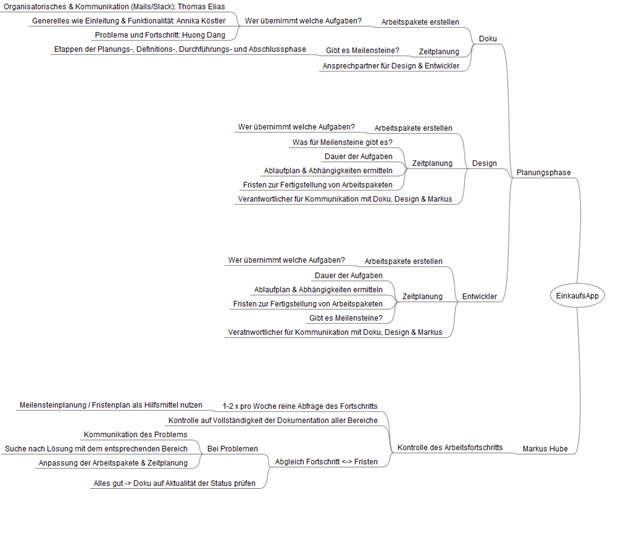
\includegraphics[scale=0.6, origin=l]{Aktivitaetsliste.png}
\\
\footnotesize Abbildung 1: Aktivitätsliste
\normalsize
\\
\linebreak
\subsubsection*{Meilensteinplanung}
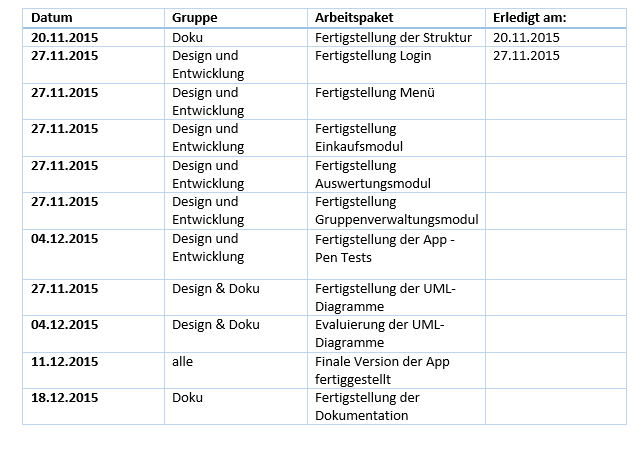
\includegraphics[scale=0.6, origin=l]{Meilensteine.png}
\\
\footnotesize Abbildung 2: Meilensteine
\normalsize
\\
\linebreak
\subsubsection*{Klassen-Diagramm}
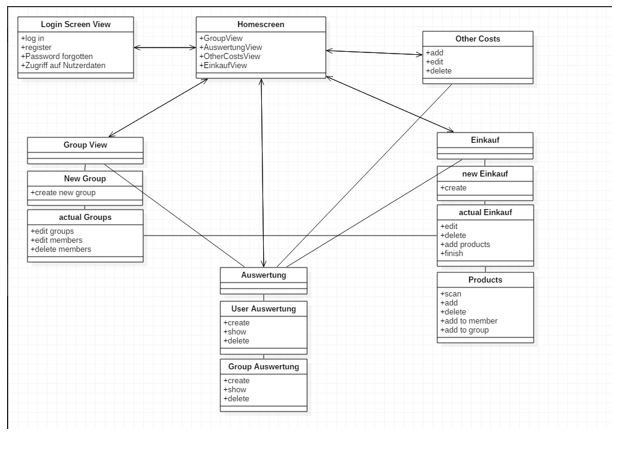
\includegraphics[scale=0.6, origin=l]{Klassendiagramm.png}
\\
\footnotesize Abbildung 3: Klassendiagramm
\normalsize
\\
\linebreak
\subsubsection*{Aktivitäts-Diagramme}
Aktivitätsdiagramm „Einkauf einlesen“ 
\\
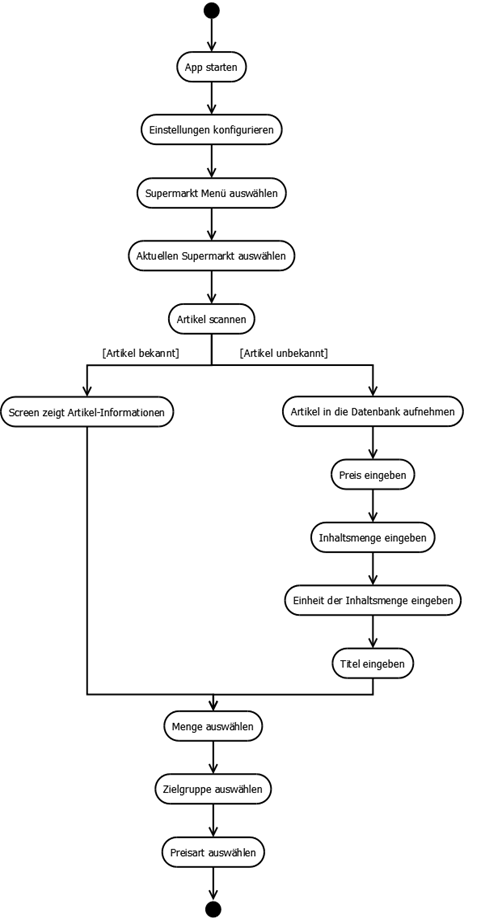
\includegraphics[scale=0.6, origin=l]{Aktivitaets-Diagramm.png}
\\
\footnotesize Abbildung 4: Aktivitätsdiagramm-Einkauf
\normalsize
\\
\newpage
Aktivitätsdiagramm „Ausgabeverlauf anzeigen“
\\
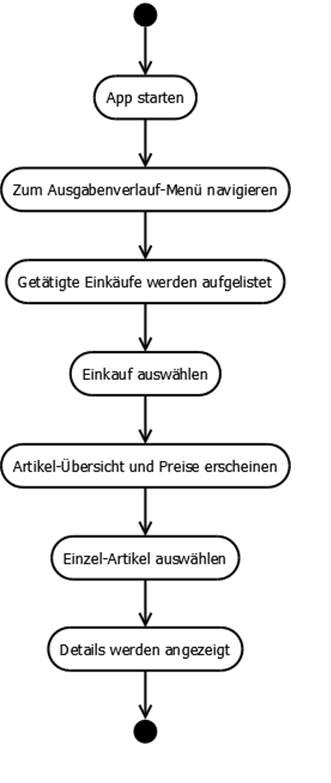
\includegraphics[scale=0.6, origin=l]{Aktivitaets-Diagramm-Ausgabenverlauf.png}
\\
\footnotesize Abbildung 5: Aktivitätsdiagramm-Ausgabenverlauf
\normalsize
\\
\linebreak
\subsubsection*{Zustandsdiagramm}
Zustands-Diagramm „Ausgabenverlauf anzeigen“
\\
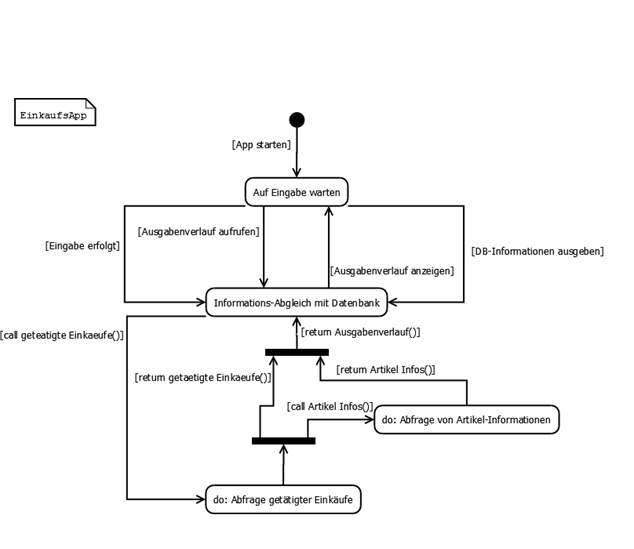
\includegraphics[scale=0.6, origin=l]{Zustandsdiagramm.png}
\\
\footnotesize Abbildung 6: Zustandsdiagramm
\normalsize
\\
\linebreak



\subsubsection{Scrum}
Nachdem ein grober organisatorischer Rahmen für das Projekt von der Gruppe Dokumentation vorgegeben wurde, haben die einzelnen Gruppen intern mittels agiler Projektmanagement-Methoden ihre Arbeitspakete und Ablaufpläne festgelegt. 
Mittels Telefonkonferenzen bei der Gruppe Dokumentation wurden Arbeitspakete erstellt und jeder hat sich nach dem Pull-Prinzip – bekannt aus der Projektmanagement-Methode Kanban – seine Arbeitspakete abgeholt und eine Bearbeitungsfrist definiert. 
In der Gruppe der Entwickler wurde unter Zuhilfenahme des Tools „Trello“ die Planung und Durchführung der Arbeitspakete durchgeführt. Trello ist ein Web-Dienst, der ein Board bietet, um Arbeitspakete gemäß agiler Projektmanagement-Methoden zu bearbeiten und Arbeitsfortschritte transparent darzustellen. 
Die Gruppe Design hat ihre Arbeitspakete auf Basis eines Ablaufplanes auf die verschiedenen Mitglieder verteilt. Es wurden die Phasen Prototyp-Entwurf, Prototyp-Review, Prototyp-Modifikationen und Prototyp-Test und Prototyp-Abnahme durchlaufen.
\newpage
\subsection{Sicherheit}
Sobald Daten eines Nutzers für eine Applikation eingefordert werden, wird ein gewisser Standard an Sicherheit gefordert. Es sollen keine Dritte an diese Daten kommen.
In der EinkaufsApp wurden folgende Maßnahmen getroffen um diese gewährleisten zu können.
Das vom Nutzer festgelegte Passwort wird als Einweg-Hash in der Datenbank gespeichert. Zudem wird in Verbindung mit dem Nutzernamen sichergestellt, dass es sich auch um den richtigen Nutzer handelt. Eine weitere wichtige Technik zur Sicherheit von Webanwendungen spielt das SSL-Protokoll (Secure Socket Layer). Bei Verwendung dieser Protokolle wird vor der eigentlichen HTTP-Kommunikation ein geschützter Kanal aufgebaut, so dass die Nutzerdaten für Dritte nicht zugängig sind. Die Nutzerdaten werden in einem normalen Web-Formular eingetragen (Login-Screen)und mittels POST-Request an den Server gesendet. Da der TCP-Kanal abgesichert ist, haben Dritte keinen Zugriff auf die Nutzdaten innerhalb des POST-Requests, d. h. Nutzername und Passwort werden gesichert übertragen. 
\newpage
\section{Durchführungsphase}
In diesem Abschnitt wird die Funktionsweise der EinkaufsApp beschrieben. Dabei werden die einzelnen Hauptprozesse einzeln vorgestellt und deren technische Umsetzung erläutert. Die Hauptprozesse sind der Login und die Registrierung des Nutzers, der Einkaufsprozess, die Nutzerverwaltung und die Auswertung. 
\subsection*{Einleitung}
\newpage
\subsection{Registrierung}
Bei der EinkaufsApp muss sich jeder Nutzer mittels einer Email-Adresse und einem Kennwort bei der App registrieren.
Eine Registrierung ist bei dieser App unentbehrlich, da für jeden Nutzer ein Profil angelegt wird und er mit diesem Profil seine Produkte einscannen kann und seine Finanzen im Blick behalten kann.
In den drei folgenden Unterpunkten wird der Prozess der Registrierung aus Seiten der Designer, Entwickler und der Dokumentation beschrieben.
\subsubsection*{Design}
Die Designer haben zu der Registrierung und zu dem Login, welcher im Punkt 3.4 behandelt wird ein Flussdiagramm entworfen, welches hier zu sehen ist.
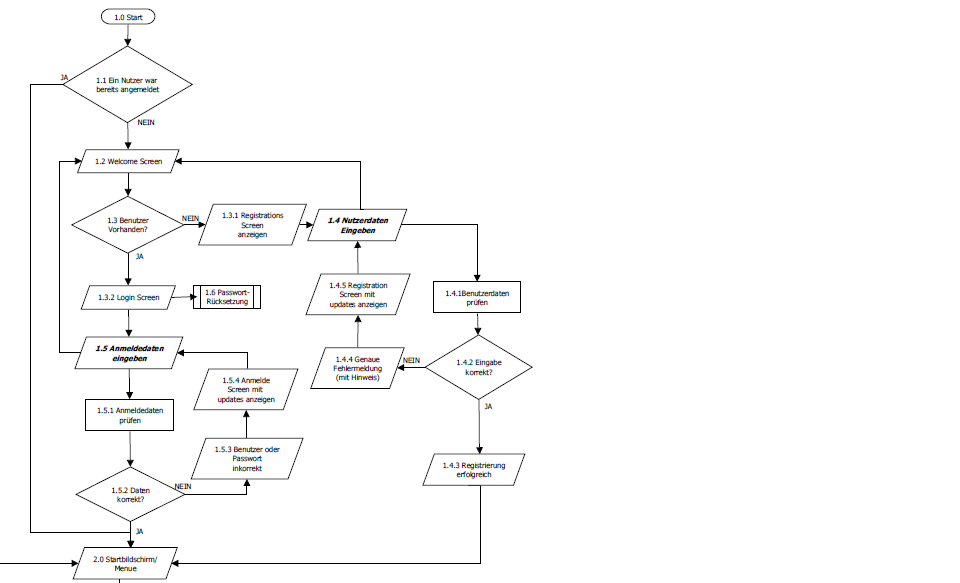
\includegraphics[scale=0.6, origin=l]{Login-Registrierung.png}
\footnotesize Abbildung 7: Flussdiagramm Login
\normalsize
\\
\linebreak
Das Flussdiagramm beschreibt sukzessiv den Ablauf des Registrierungs- und des Loginvorgangs, welcher von den Entwicklern umgesetzt wurde.
\subsubsection*{Entwicklung}
%Diagramm?
Die Entwickler befassen sich mit den Funktionen der Applikation  und sorgen bei der Registrierung dafür, dass alle Daten ordentlich geprüft und in die Datenbank eingepflegt werden.
Als Datenbank wird die MongoDB genutzt und via RoboMongo gemanagt. Als Programmiersprache wird in allen, auch den folgenden Unterpunkten JavaScript verwendet.
Bei der Registrierung werden die einzelnen Benutzereingaben durch bestimmte Regeln auf z.B. Länge, Email-Format, Eindeutigkeit, sowie Sicherheitskriterien der Passwortvergabe in der Applikation geprüft.
% Konkrete Regeln siehe Handbuch
Wenn alle Prüfungen erfolgreich waren, wird der Benutzer angelegt und das Passwort verschlüsselt in Form eines Hashs in der Datenbank gespeichert.
\subsubsection*{Problembeschreibung} 
Eine ganz wichtige und entscheidende Rolle spielt hierbei der Datenschutz und die Datensicherheit. Alle eingetragenen Daten des Nutzers müssen abgesichert sein, sodass kein Dritter sich an diesen Daten vergreifen kann.
\newpage
\subsubsection{Login}
\subsubsection*{Design}
Das Flussdiagramm der Designer für den Login ist im Abschnitt 3.3 Registrierung zu finden. 
\subsubsection*{Entwicklung}
Die Entwicklung beschäftigt sich mit der Funktionsweise des Logins und prüft hierbei, ob der Benutzer in der Datenbank existiert. Falls dies der Fall ist, wird das Passwort geprüft und bei korrekter Eingabe ist der Login erfolgreich durchgeführt.
Wenn der Benutzer sein Passwort vergessen hat, kann er dieses zurücksetzen lassen. Hierbei bekommt er eine E-Mail an die im Userprofil hinterlegte E-Mail Adresse. Diese enthält ein Token womit es einen Benutzer ermöglicht wird sein Passwort zu ändern. Dieses Token ist genau eine Stunde gültig, danach verfällt es. 
Nachdem der Nutzer sein Passwort zweimal eintragen musste, ändert die Datenbank das Kennwort des Nutzer und speichert dieses.
\subsubsection*{Problembeschreibung} --> Probleme beschreiben
Fehler bei Passwortrücksetzung weil Email nicht verschickt wird.
\newpage


\subsection{Einkauf}
Gruppeneinkauf vereinfacht, Einkauf fortsetzen eingebaut und Passwort rücksetzen
Gruppenverwaltung wurde zu Verwaltung allgemein:  Verwaltung von Gruppen UND KONTAKTE 
Kontaktverwaltung wird noch erstellt"
\subsubsection*{Design}
\subsubsection*{Entwicklung}
\subsubsection*{Dokumentation} --> Probleme beschreiben
\newpage

\subsection{Nutzerverwaltung}
Die Nutzerverwaltung ermöglicht dem Nutzer die individuelle Zuweisung von Artikeln an einzelne Gruppenmitglieder einer zuvor erstellten Gruppe. Ziel dessen ist die vereinfachte Finanzverwaltung.

\subsubsection*{Design}
(insert Flussdiagramm Gruppenverwaltung)
Die Gruppenverwaltung wird in zwei Teile unterteilt. Der Erste beschreibt die Gruppenerstellung. Wie im Flussdiagramm zu sehen, kann eine Gruppe angelegt werden indem zunächst der Nutzer die Menüoption Mitgliederliste wählt und hier eine Gruppe erstellt. Dabei können Mitglieder hinzugefügt bzw. auch gelöscht werden.
\subsubsection*{Entwicklung}

\subsubsection*{Dokumentation} --> Probleme beschreiben
\newpage

\subsection{Auswertung}
Der Nutzer hat die Möglichkeit vergangene Einkäufe auswerten zu lassen. Dabei hat er unterschiedliche Möglichkeiten.  Es gibt die zeitliche Eingrenzung, eine Artikeleingrenzung und eine Gruppenmitgliedereingrenzung, bei der alle vergangenen Einkäufe von bestimmten Gruppen zusammengefasst werden.
\subsubsection*{Design}
(insert Auswertungsdia)
\subsubsection*{Entwicklung}

\subsubsection*{Dokumentation} --> Probleme beschreiben
\newpage

\section{Problemzusammenfassung}
%Hier wird das Ergebnis beschrieben.
\subsection{Usability der App}
\newpage
\subsection{Organisation Projektmanagement}
\newpage
\section{Projektabschluss}
\subsection{Fertiges Produkt}
\subsection{Aussichten}
nicht umgesetzte Ideen --> siehe Excelliste
\newpage
\subsection{Zusammenfassung}
\newpage
\section{Lesson learned}
\newpage
\section*{Quellen}
\addcontentsline{toc}{section}{Quellen}
\subsection*{Internetquellen}
\begin{itemize}
\item[1.]Ionic Framework: \url{http://ionicframework.com/}
\item[2.]Ionic Guide: \url{http://ionicframework.com/docs/guide/}
\item[3.]Ionic Getting Started: \url{http://ionicframework.com/getting-started/}
\item[4.]ngCordova - Plugin Seite \url{http://ngcordova.com/}
\item[5.]BarCode Scanner : Plugin \url{hhttp://ngcordova.com/docs/plugins/barcodeScanner/}
\item[6.]Beispiel Projekt: \url{https://github.com/bastisk/suedm}
\item[7.]Editor: \url{http://brackets.io/}
\item[8.]Angular JS-Kurs: \url{https://www.codeschool.com/courses/shaping-up-with-angular-js/}
\item[9.]Tutorial zum Routing: \url{https://scotch.io/tutorials/angular-routing-using-ui-router}
\item[10.]App-Projekt: \url{http://www.mobile2b.de/ablauf-app-projekt/}
\item[11.] Dokumentationshilfe: \url{http://www.tellsbells.de/dokuwebsite/tbdokumentation.pdf}
\item[12.] Dokumentationshilfe: \url{https://www.lecturio.de/magazin/projekte-dokumentieren/}
\item[13.] Open Source mit API über eine einfachen HTTP-GET-Reguest: \url{http://www.opengtindb.org/api.php}
\item[14.] Suchmaschine der Firma die GTIN-Nummern verwaltet: \url{http://www.gepir.de/v31/V31_client/gtin.aspx}
\end{itemize}

\newpage
\section*{Organisationstool- Übersicht}
\begin{itemize}
\item[-]Allgemeine Ablage: GitHub
\item[-]Diskussionsrunden: Slack
\item[-]Informationsaustausch: via Email
\item[-]Diagramme zeichen: via Dia 
\item[-]Kreieren von Web-Prototypen: proto.io
\item[-]Datenbanken und Datenbankenverwaltung: MongoDB, RoboMongo
\end{itemize}
\newpage
\section*{Anhang}
\addcontentsline{toc}{section}{Anhang}

\end{document}

    Status API Training Shop Blog About Pricing 

    © 2015 GitHub, Inc. Terms Privacy Security Contact Help 
